% Paquets généraux
\documentclass[a4paper,12pt,titlepage]{article}
\usepackage[T1]{fontenc}
\usepackage[utf8]{inputenc}
\usepackage[french]{babel}
\usepackage[gen]{eurosym}
%\usepackage[dvips]{graphicx}
\usepackage{fancyhdr}
\usepackage{pdfpages} 
\usepackage{multido}
\usepackage{moreverb}
\usepackage{hyperref}
%\usepackage{textcomp}
\usepackage{verbatim}
\usepackage{moreverb}
\usepackage{listings}
\usepackage{minted}
\usepackage{eso-pic}
\usepackage{enumitem}
\usepackage{comment}
\usepackage{boxedminipage}
\usepackage[french,onelanguage, boxruled,linesnumbered]{algorithm2e}


\newcommand{\auteurun}{Juliette Genzmer}
\newcommand{\auteurdeux}{Willie Robert}
\newcommand{\auteurtrois}{Renaud Costadoat}
\newcommand{\institute}{Lycée Dorian}
\newtheorem{solution}{Solution}


\newcommand{\nom}{Porte conteneur}
\newcommand{\sequence}{03}
\newcommand{\num}{04}
\newcommand{\type}{TD}
\newcommand{\descrip}{Résolution d'un problème en utilisant des méthodes algorithmiques}
\newcommand{\competences}{Alt-C3: Concevoir un algorithme répondant à un problème précisément posé}

\usepackage{color}
\usepackage{xcolor}
\usepackage{colortbl}
\usepackage{helvet}
\renewcommand{\familydefault}{\sfdefault}
\usepackage{amsfonts}
\usepackage{amsmath}
%\usepackage{xspace}
\usepackage{varioref}
\usepackage{tabularx}
%\usepackage{floatflt}
\usepackage{graphics}
\usepackage{wrapfig}
\usepackage{textcomp}
\usepackage{tikz}
\usepackage{wrapfig}
\usepackage{gensymb}
\usepackage{ifthen}
\usepackage{cancel}
\usepackage{etoolbox}
\usepackage{multirow}
%\usepackage{boxedminipage}
\definecolor{gris25}{gray}{0.75}
\definecolor{bleu}{RGB}{18,33,98}
\definecolor{bleuf}{RGB}{42,94,171}
\definecolor{bleuc}{RGB}{231,239,247}
\definecolor{rougef}{RGB}{185,18,27}
\definecolor{rougec}{RGB}{255,188,204}%255,230,231
\definecolor{vertf}{RGB}{103,126,82}
\definecolor{vertc}{RGB}{220,255,191}
\definecolor{forestgreen}{rgb}{0.13,0.54,0.13}
\definecolor{blcr}{rgb}{0.59,0.69,0.84}
\definecolor{blfr}{rgb}{0.32,0.51,0.75}
\definecolor{orfr}{rgb}{0.90,0.42,0.15}
\definecolor{orcr}{rgb}{0.90,0.65,0.50}
\definecolor{orangef}{rgb}{0.659,0.269,0.072}
\definecolor{orange}{rgb}{0.58,0.35,0.063}
\definecolor{orangec}{rgb}{0.43,0.32,0.25}
\definecolor{rcorrect}{rgb}{0.6,0,0}
\definecolor{sequence}{rgb}{0.75,0.75,0.75}
\definecolor{competences}{rgb}{0.61,0.73,0.35}
\definecolor{grisf}{HTML}{222222}
\definecolor{grisc}{HTML}{636363}
\definecolor{normal}{HTML}{4087c4}
\definecolor{info}{HTML}{5bc0de}
\definecolor{success}{RGB}{92,184,92}
\definecolor{warning}{RGB}{240,173,78}
\definecolor{danger}{RGB}{217,83,79}
\hypersetup{                    % parametrage des hyperliens
    colorlinks=true,                % colorise les liens
    breaklinks=true,                % permet les retours à la ligne pour les liens trop longs
    urlcolor= blfr,                 % couleur des hyperliens
    linkcolor= orange,                % couleur des liens internes aux documents (index, figures, tableaux, equations,...)
    citecolor= forestgreen                % couleur des liens vers les references bibliographiques
    }

% Mise en page
\pagestyle{fancy}

\setlength{\hoffset}{-18pt}

\setlength{\oddsidemargin}{0pt} 	% Marge gauche sur pages impaires
\setlength{\evensidemargin}{0pt} 	% Marge gauche sur pages paires
\setlength{\marginparwidth}{00pt} 	% Largeur de note dans la marge
\setlength{\headwidth}{481pt} 	 	% Largeur de la zone de tête (17cm)
\setlength{\textwidth}{481pt} 	 	% Largeur de la zone de texte (17cm)
\setlength{\voffset}{-18pt} 		% Bon pour DOS
\setlength{\marginparsep}{7pt}	 	% Séparation de la marge
\setlength{\topmargin}{-30pt} 		% Pas de marge en haut
\setlength{\headheight}{55pt} 		% Haut de page
\setlength{\headsep}{20pt} 		% Entre le haut de page et le texte
\setlength{\footskip}{30pt} 		% Bas de page + séparation
\setlength{\textheight}{700pt} 		% Hauteur de l'icone zone de texte (25cm)
\setlength\fboxrule{1 pt}
\renewcommand{\baselinestretch}{1}
\setcounter{tocdepth}{1}
\newcommand{\cadre}[2]
{\fbox{
  \begin{minipage}{#1\linewidth}
   \begin{center}
    #2\\
   \end{center}
  \end{minipage}
 }
}

\newcounter{num_quest} \setcounter{num_quest}{0}
\newcounter{num_rep} \setcounter{num_rep}{0}
\newcounter{num_cor} \setcounter{num_cor}{0}

\newcommand{\question}[1]{\refstepcounter{num_quest}\par
~\ \\ \parbox[t][][t]{0.15\linewidth}{\textbf{Question \arabic{num_quest}}}\parbox[t][][t]{0.85\linewidth}{#1\label{q\the\value{num_quest}}}\par\par
}



\newcommand{\reponse}[0]{\refstepcounter{num_rep}\par
~\ \\ \parbox[t][][t]{0.15\linewidth}{\textbf{Question \arabic{num_rep}}}}

\newcommand{\cor}
{\refstepcounter{num_cor}
\noindent
\rule{\linewidth}{.5pt}
\textbf{Question \arabic{num_cor}:} \\
}



% En tête et pied de page
\lhead{\nom}
\rhead{
\includegraphics[width=2cm]{../../../img/logo}}
\lfoot{David Aubert, Renaud Costadoat}
\rfoot{Page \thepage}
\cfoot{}

\newlength{\RoundedBoxWidth}
\newsavebox{\GrayRoundedBox}
\newenvironment{GrayBox}[1][\dimexpr\textwidth-4.5ex]%
   {\setlength{\RoundedBoxWidth}{\dimexpr#1}
    \begin{lrbox}{\GrayRoundedBox}
       \begin{minipage}{\RoundedBoxWidth}}%
   {   \end{minipage}
    \end{lrbox}
    \begin{center}
    \begin{tikzpicture}%
       \draw node[draw=bleuf,fill=bleuc,rounded corners,%
             inner sep=2ex,text width=\RoundedBoxWidth]%
             {\usebox{\GrayRoundedBox}};
    \end{tikzpicture}
    \end{center}}

\fancypagestyle{correction}{%
  \fancyhf{}
  \lhead{\colorbox{danger}{\begin{minipage}{0.65\paperwidth} \textcolor{white}{\textbf{Correction}} \end{minipage}} }
  \rhead{
\includegraphics[width=2cm]{../../../img/logo}}
  \lfoot{Juliette Genzmer, Willie Robert, Renaud Costadoat}
  \rfoot{\colorbox{danger}{\begin{minipage}{0.3\paperwidth} \begin{flushright}\textcolor{white}{\textbf{Correction}}\end{flushright} \end{minipage}} }}

\renewcommand{\footrulewidth}{0.4pt}


\newcommand{\BackgroundPic}{%
\put(0,0){%
\parbox[b][\paperheight]{\paperwidth}{%
\vfill
\begin{center}
\hspace{0.5cm}\vspace{0.5cm}

\includegraphics[width=\paperwidth,height=\paperheight,%
keepaspectratio]{../../../img/fond5}%
\end{center}
\vfill
}}}

\newcommand{\goforum}{
\begin{figure}[ht!]
\begin{center}
 
\includegraphics[width=0.7\linewidth]{../../../img/go_forum}
\end{center}
\label{go_forum}
\caption{J'pète les plombs}
\end{figure}}

\newcommand{\BackgroundPicdeux}{%
\put(25,-30){%
\parbox[b][\paperheight]{\paperwidth}{%
\vfill
\begin{center}

\includegraphics[width=\paperwidth,height=\paperheight,%
keepaspectratio]{../../../img/fond6}%
\end{center}
\vfill
}}}

\setenumerate[1]{align=left,label=\arabic*}
\setenumerate[2]{before=\stepcounter{enumi},label*=.\arabic*,leftmargin=1.2em,align=left}

\begin{document}


\pagestyle{fancy}

\AddToShipoutPicture{\BackgroundPicdeux}

\begin{center}
{\Large\bf {\type} \no {\numero} -- \descrip}
\end{center}

\SetKw{KwFrom}{de} 

\begin{boxedminipage}{.9\textwidth} 
\begin{itemize}
 \item Faire tous les exercices dans un fichier {NomPrenom.py} à sauvegarder,
 \item mettre en commentaire l'exercice et la question traités (ex: \# Exercice 1),
 \item ne pas oublier pas de commenter ce qui est fait dans votre code (ex: \# Je crée une fonction pour calculer la racine d'un nombre),
 \item il est possible de demander un déblocage pour une question, mais celle-ci sera notée 0,
 \item il faut vérifier avant de partir que le code peut s'exécuter et qu'il affiche les résultats que vous attendez. Les lignes de code qui doivent s'exécuter sont décommentées.
\end{itemize}
\end{boxedminipage}

\section{Gradient de couleur en spirale}

En géométrie plane, les spirales forment une famille de courbes d'allure similaire : une partie de la courbe semble s'approcher d'un point fixe tout en tournant autour de lui, tandis que l'autre extrémité semble s'en éloigner. 

	Le premier but de cet exercice est de tracer le gradient de couleur (du rouge vers le vert) en spirale, comme sur la figure \ref{fig01}.

\begin{figure}[!ht]
\centering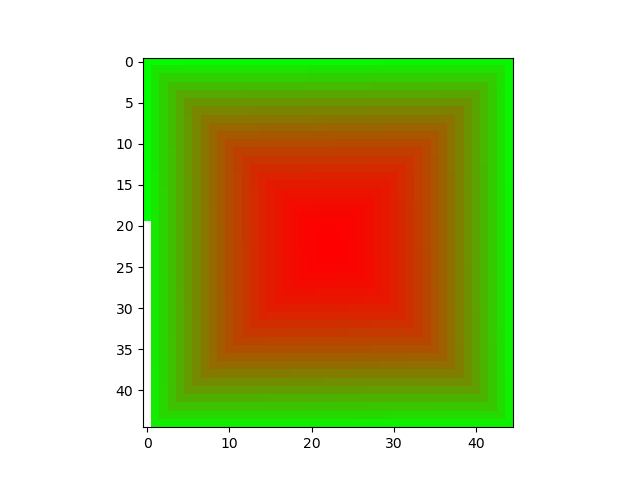
\includegraphics[width=0.8\linewidth]{img/fig01}
\caption{\label{fig01} Gradient de couleur en spirale }
\end{figure}

Le code suivant permet de tracer cette spirale colorée (les commentaires dont les lignes qui commencent par \# ne sont pas obligatoires, sauf la première ligne \texttt{\# -*- coding: utf-8 -*-}).
 
\newpage

\begin{minted}[linenos]{python}
# -*- coding: utf-8 -*-

# Import des bibliotheques
import numpy as np
import matplotlib.pyplot as plt
import matplotlib as mpl

# Fonction qui détermine la couleur d'un pixel
# en fonction de sa position
def colorFader(mix=0):
    c1=np.array([1,0,0])
    c2=np.array([0,1,0])
    return (1-mix)*c1 + mix*c2

# Parcours de la spirale a partir du centre
# en fonction de la valeur de entier
# a recopier pour la question 1 et à copier et
# modifier pour la question 3
max=2000
imagebase = np.ones([int(max**0.5)+1,int(max**0.5)+1,3])
coords=[0,0]
i=0
entier=0
while entier<max:
    entier+=1
    # le pixel de imagebase qui a pour coordonnées
    # [coords[0]+(int(max**0.5))//2,coords[1]+(int(max**0.5))//2]
    # est coloré avec une couleur déterminée par la fonction colorFader
    dec=(int(max**0.5))//2
    imagebase[coords[0]+dec,coords[1]+dec]=colorFader(entier/max)
    # on passe ensuite au pixel suivant pour parcourir toute la spirale
    if coords==[i,-i]:
        coords[0]+=1
        i+=1
    elif coords[0]==i and coords[1]<i:
        coords[1]+=1
    elif coords[0]>-i and coords[1]==i:
        coords[0]-=1
    elif coords[0]==-i and coords[1]>-i:
        coords[1]-=1
    elif coords[0]<i and coords[1]==-i:
        coords[0]+=1

# Tracé de la figure de la réponse
plt.imshow(imagebase)
plt.show()
\end{minted}

\question{Recopier le code précédent et exécuter le script. La figure \ref{fig01} doit alors apparaître (Si ce n'est pas le cas, la console python vous indique la ligne où vous avez fait une erreur)?}

\section{Parité des nombres}

On donne le code suivant:
\begin{minted}{python}
def est_pair(n):
    return n%2==1

print(est_pair(3))
\end{minted}

Cette fonction ne renvoie pas ce qui est prévu, c'est à dire :
\begin{itemize}
 \item \texttt{True} si le nombre est pair,
 \item \texttt{False} si le nombre est impair.
\end{itemize}

\question{Recopier et corriger le code précédent pour que la fonction \texttt{est\_pair(n)} ne renvoie \texttt{True} que si le nombre est pair.}

~\

\begin{figure}[!ht]
\begin{minipage}{0.45\linewidth}
On souhaite réaliser la figure \ref{fig02} dont les pixels sont colorés selon le principe suivant:
\begin{itemize}
 \item si \texttt{entier} est pair alors le pixel doit être noir:\\ \texttt{imagebase[coords[0]+dec,coords[1]+dec]=
 [0,0,0]},
 \item si \texttt{entier} est impair alors on ne fait rien, on laisse le pixel blanc.
\end{itemize}
\end{minipage}\hfill
\begin{minipage}{0.45\linewidth}
\centering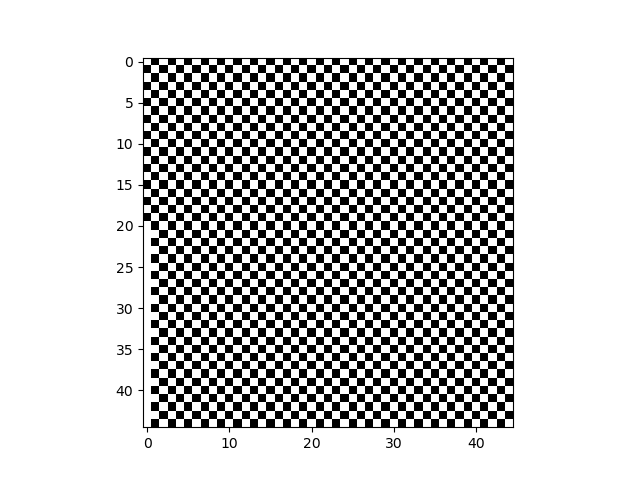
\includegraphics[width=0.9\linewidth]{img/fig02}
\caption{\label{fig02} Coloration de la figure en fonction de la parité de \texttt{entier}}
\end{minipage}
\end{figure}

\question{Recopier et modifier les lignes 15 à 46 (sans les commentaires) afin de réaliser la figure \ref{fig02}}

\section{La spirale d'Ulam}

En mathématiques, la spirale d'Ulam, ou spirale des nombres premiers (dans d'autres langues, elle est appelée aussi horloge d'Ulam) est une méthode simple pour la représentation des nombres premiers qui révèle un motif qui n'a jamais été pleinement expliqué. Elle fut découverte par le mathématicien Stanislaw Ulam, lors d'une conférence scientifique en 1963. 

\newpage

Un algorithme pour décider si un nombre est premier (appelés tests de primalité) consiste à essayer de le diviser par tous les nombres en commençant par 2, qui n'excèdent pas sa racine carrée : s'il est divisible par l'un d'entre eux, il est composé, et sinon, il est premier.

~\

Ainsi la fonction à coder est la suivante:
\begin{enumerate}
\item Si n est strictement inférieur à 2, il est premier \texttt{return True},
\item Sinon:
\begin{enumerate}
\item on initialise d : \texttt{d=2},
\item tant que d est inférieur ou égal à la racine carrée de n : \texttt{d<=n**0.5},
\begin{enumerate}
\item si le reste de la division euclidienne de n par d faut 0 : \texttt{n\%d==0},
\item alors le nombre n'est pas premier, je retourne un False : \texttt{return False},
\item sinon j'ajoute 1 à d : \texttt{d+=1}.
\end{enumerate}
\item Le nombre est premier si aucun d n'est un diviseur de n \texttt{return True}.
\end{enumerate}
\end{enumerate}

\question{Coder la fonction \texttt{est\_premier(n)} à partir de cet algorithme. Elle doit renvoyer \texttt{True} si \texttt{n} est premier, \texttt{False} sinon.}

~\

On souhaite réaliser la figure \ref{fig03} dont les pixels sont colorés selon le principe suivant:
\begin{itemize}
 \item si \texttt{entier} est premier alors le pixel doit être noir:\\ \texttt{imagebase[coords[0]+dec,coords[1]+dec]=[0,0,0]},
 \item si \texttt{entier} est composé alors on ne fait rien, on laisse le pixel blanc.
\end{itemize}


\begin{figure}[!ht]
\centering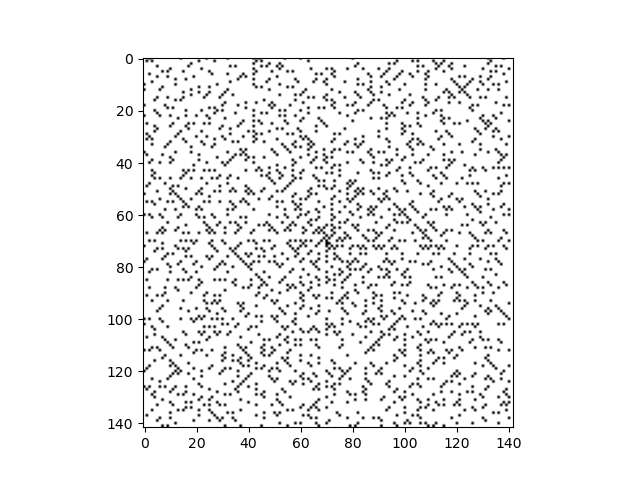
\includegraphics[width=0.7\linewidth]{img/fig03}
\caption{\label{fig03} Coloration de la figure en fonction du fait que \texttt{entier} soit premier}
\end{figure}

\question{Recopier les modifier les lignes 15 à 46 (sans les commentaires) afin de réaliser la figure \ref{fig03}. La valeur max devra être de 20000 pour cette question.}

\begin{center}
\Large{FIN}
\end{center}

\cleardoublepage

\ifdef{\public}{\end{document}}{\pagestyle{correction}}

\begin{center}
\Large{Correction}
\end{center}

\reponse{}

Recopier le code.

\reponse{}

\begin{minted}{python}
def est_pair(n):
    return n%2==0

print(est_pair(3),est_pair(4))
\end{minted}

\reponse{}

\begin{minted}{python}
# Parcours de la spirale a partir du centre
# en fonction de la valeur de entier
max=2000
imagebase = np.ones([int(max**0.5)+1,int(max**0.5)+1,3])
coords=[0,0]
i=0
entier=0
while entier<max:
    entier+=1
    # le pixel de imagebase qui a pour coordonnées
    # [coords[0]+(int(max**0.5))//2,coords[1]+(int(max**0.5))//2]
    # est coloré avec une couleur déterminée par la fonction colorFader
    if est_pair(entier):
        dec=(int(max**0.5))//2
        imagebase[coords[0]+dec,coords[1]+dec]=[0,0,0]
    if coords==[i,-i]:
        coords[0]+=1
        i+=1
    elif coords[0]==i and coords[1]<i:
        coords[1]+=1
    elif coords[0]>-i and coords[1]==i:
        coords[0]-=1
    elif coords[0]==-i and coords[1]>-i:
        coords[1]-=1
    elif coords[0]<i and coords[1]==-i:
        coords[0]+=1

# Tracé de la figure de la réponse
plt.imshow(imagebase)
plt.show()
\end{minted}

\newpage

\reponse{}

\begin{minted}{python}
def est_premier(n):
    if n <2:
        return True
    d=2
    while d<=n**0.5:
        if n%d==0:
            return False
        else:
            d+=1
    return True

print(est_premier(6),est_premier(37))
\end{minted}


\reponse{}

\begin{minted}{python}
# Parcours de la spirale a partir du centre
# en fonction de la valeur de entier
max=20000
imagebase = np.ones([int(max**0.5)+1,int(max**0.5)+1,3])
coords=[0,0]
i=0
entier=0
while entier<max:
    entier+=1
    # le pixel de imagebase qui a pour coordonnées
    # [coords[0]+(int(max**0.5))//2,coords[1]+(int(max**0.5))//2]
    # est coloré avec une couleur déterminée par la fonction colorFader
    if est_premier(entier):
        dec=(int(max**0.5))//2
        imagebase[coords[0]+dec,coords[1]+dec]=[0,0,0]
    if coords==[i,-i]:
        coords[0]+=1
        i+=1
    elif coords[0]==i and coords[1]<i:
        coords[1]+=1
    elif coords[0]>-i and coords[1]==i:
        coords[0]-=1
    elif coords[0]==-i and coords[1]>-i:
        coords[1]-=1
    elif coords[0]<i and coords[1]==-i:
        coords[0]+=1

# Tracé de la figure de la réponse
plt.imshow(imagebase)
plt.show()
\end{minted}

\end{document}
